\section{VOICESCRIPT Authoring Interface}

Based on these observations, we developed \systemname, a speech authoring interface that supports script writing, speech recording and audio editing in a single unified workflow. Our interface is built on two key features.

\begin{figure*}
  \centering
  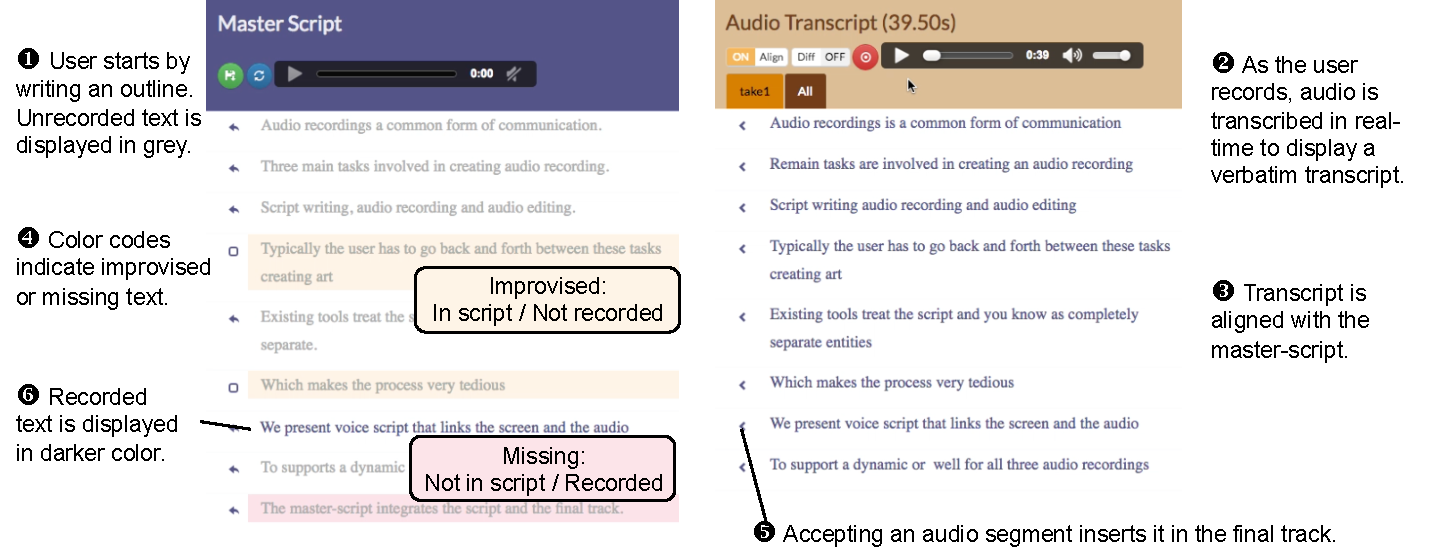
\includegraphics[width=2.0\columnwidth]{figures/ui_aligned}
  \caption{The \systemname\ interface. The \textit{master-script} view on the left shows the current state of the project, including both recorded and unrecorded text. On the right, there are individual tabs for each recording, along with an \textit{All} tab that shows transcribed text from all takes.}~\label{fig:ui_aligned}
\end{figure*}

\textbf{Text-based representation of audio.} We build on previous work~\cite{casares2002simplifying,whittaker2004semantic,berthouzoz2012tools,rubin2013content} that demonstrates the benefits of text-based representations of spoken audio for navigation and editing. \systemname\ uses automatic speech recognition (ASR) to transcribe audio recordings in realtime and represent each take with a verbatim transcript. As with previous systems, edits to these text transcripts are automatically propagated to the audio, which facilitates simple audio editing tasks. 

\textbf{Master-script view.} To help users manage the relationship between scripted text and recorded speech, we introduce the notion of a \emph{master-script} that shows a unified view of both unrecorded portions of the script and recorded speech to include in the final track. By representing and visualizing both recorded and unrecorded text, the master-script provides a complete, readable view of the current state of the project that evolves as the user records and adds new takes to the final track, edits recorded text, or adds/modifies text that must be recorded. 

\textbf{Merge process.} Since recorded text typically differs from the script, \systemname\ provides an interface for merging changes into the master-script. The fact that we represent all recorded audio as text allows us to use standard text differencing to identify conflicts and execute merges. One key difference between our scenario and standard text merging is that recorded audio cannot simply be cut and merged into the master-script at any arbitrary word boundary. In many cases, the temporal gap between spoken words is not big enough to produce a seamless edit in the final track. Our merge interface takes this into account and helps the user execute merges that are likely to be artifact-free.

% As shown in Figure~\ref{interface}, our interface consists of two types of documents: a \textit{Master Script} document (left) displays the current status of the final track, including what has been recorded and what was planned to be recorded but has not been recorded yet (i.e. the original script), while a \textit{Transcript} document (right) displays the verbatim transcript of individual audio takes. As the user records new takes, our tool aligns the audio transcripts to the master script so that it is easy to compare each take with the master script and with each other. It also partitions each recording into segments that can be seamlessly joined between takes. At any point during the recording process, the user can edit the script or the final track by editing the master script like a text document.

\subsection{Interface and Usage Scenario}
The rest of this section describes our interface using an example scenario of how a user might create an audio recording. 

Typically, the user begins by writing an outline of points to record in the master-script.
The text appears in light grey to indicate that these parts have not been recorded yet (Figure~\ref{fig:ui_aligned} \textit{left}). At this stage, the master-script is like an ordinary, editable text document. 

Once the user starts recording, the audio is transcribed in real time and verbatim text corresponding to each take appears in a separate transcript tab (Figure~\ref{fig:ui_aligned} \textit{right}). Each transcript is time-aligned with the corresponding recording, so the user can quickly navigate to specific
parts of the audio by clicking on a word in the transcript. 

The next task is to decide which parts of the recording to merge into the master-script. To this end, we provide a \textit{compare-view} that aligns segments of the recording transcript to corresponding segments in the master-script and shows them side-by-side. To emphasize discrepancies between the script and recording, the user can enable a \textit{diff-view} that displays per-word differences using standard track change markers (i.e., strike throughs for missing words and highlighting for added words). Any segment of the transcript that does not correspond to any part of the master-script (e.g., where the speaker improvised) is highlighted in yellow in the transcript tab. To add recorded audio to the final track, the user can \textit{accept} any portion of the recording by clicking a button next to the appropriate transcript segment. If there is a corresponding segment in the master-script, the accepted transcript segment replaces it. If there is no corresponding master-script segment, the accepted transcript segment is simply inserted into the master-script. Within the master-script, accepted segments appear in black to indicate that these are recorded portions of text that have been added to the final track. 

If the user records multiple takes, in addition to each of the transcript tabs, the \textit{All} tab provides a summary of all of the takes. For each segment in the master script, this tab displays all the corresponding transcript segments from all of the audio takes. A drop-down button next to a transcript segment  indicates that there are multiple versions (or takes)  of the  segment. Clicking on the button opens a list showing the alternative versions (Figure ~\ref{fig:multipletakes}). The user can listen to any of these takes and select one without having to search through individual takes. When the All tab is in focus, any part of the master-script that has not been recorded in any of the takes is highlighted in red. In this way, the user can tell at a glance what has already been recorded and what still needs to be recorded. All of the dark (i.e. recorded) text in the master-script represents the current state of the final audio track; all of the grey text that is not highlighted in red has been recorded but the author has not yet accepted it into the final track. 

During any point in the process, the user can edit the master-script like a text document.  For example, the user can simply insert more text to record, or make changes to unrecorded text to flesh out the original outline or change the wording of a particular sentence. If the user deletes a recorded word from the text, it will be deleted from the final track. The user can also correct the transcription of a recorded word without affecting the underlying audio. When the user edits a recorded word (without completely deleting it), the word is italicized and marked red to warn the user that it may no longer match the underlying audio. If the edit was made to correction a transcription error and the word does indeed match the audio, the user can manually mark the word as \textit{clean} which returns it to a normal dark font. If the edit was intended to change the content, the user can use the mark as a reminder to re-record that portion of the audio.
\begin{figure}
\centering
  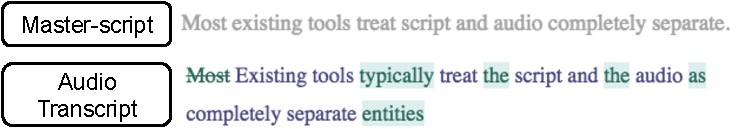
\includegraphics[width=1.0\columnwidth]{figures/diffview}
  \caption{The \textit{diff-view} displays a per-word difference between the master-script and the audio transcript.}~\label{fig:diffview}
\end{figure}

% \VTODO{Instead of describing all the different text colors throughout the section, it might be a bit clearer to skip all descriptions of text colors above and add a paragraph here saying that we visualize the text in the master-script with different colors to help users understand the state of the document. Red mean unrecorded, dark is accepted, etc.}

In order to produce the final recording, the user iterates back and forth between all of these operations, editing the master-script, recording audio takes, comparing alternative takes and accepting audio segments into the final track.
One key benefit of our interface is that it supports a wide range of workflows for different users and scenarios. For instance, instead of starting with a written outline, the user can begin with an empty master-script, start recording, and then use  the initial recording as an outline. The user can also record the entire script in a single take, or work on a single section at a time. 
